\chapter{General Information}

\section{Reading in data files}
When you are trying to cluster and classify data, typically the first step is reading in the data from a file. There are several different ways that data is typically stored in a data file, the most common formats are comma separated values (csv) or tab separated values (tsv). For both of these types of files, R has some inbuilt functions for reading them into data frames.

Typically csv files tend to be easier to read in, as they usually have proper column labels and very simple value separation. Tsv files can vary in their formatting between tabs and different types of spacing, and often do not have column labels.

\subsection{CSV files}
Csv files are very easy to read in with R. Let's consider the following csv file.

\begin{verbatim}
id,mag,amp,error
00001,20.123,19.312,0.2486362
00003,19.02,20.2,0.47823
00004,18.8,21.389,0.277669
\end{verbatim}

In R you can read in csv files using the \verb|read.csv| function. We must note that this csv file has column headers, so we need to add an argument to indicate this.

\begin{verbatim}
myData <- read.csv("data.csv", header=TRUE)
\end{verbatim}

\subsection{TSV files}
Let's take a look at a more unusual tsv file and read it in to R. This tsv file uses a special format that allocates a specific width to each column, such that a non-standard amount of additional spaces are added for padding.

\begin{verbatim}
00001  20.123 19.312  0.2486362
00003  19.023 20.213  0.4782373
00004  18.789 21.389  0.2776688
\end{verbatim}

To read this data in with R we need to use the \verb|read.table| function. We must note that the data file does not have column headers, and does not have a sepcific separater string.

\begin{verbatim}
myData <- read.table("data.tsv")
\end{verbatim}

The resulting data frame will include all of the given data, however its column names with be generic. The next thing we will need to do is to label the columns. In R there are many different ways to rename columns, however since we want to rename all of the columns we can make use of the \verb|names| function.

\begin{verbatim}
names(myData) <- c("id", "mag", "amp", "error")
\end{verbatim}

\section{Plotting data}
Once you have read in your data it is always a good idea to visualize your data to get a general idea of what it looks like and how it might cluster. How you should visualize your data depends on how many features it has and what features of it you want to look at.

If you just want to look at one or two features, you can use the \verb|ggplot2| library to create plots of your data. The exact type of graph that you should use will depend on the data, but usually a scatter plot is a good first choice.

If you want to look at three features of your data at the same time, you can use the \verb|plotly| library to visualize it. The library offers good 3d scatter plots that can be very useful.

\subsection{plotly}
The \verb|plotly| library is a good library for plotting 3d data graphs. In particular the 3d scatter plots that it offers are very useful.

\begin{center}
	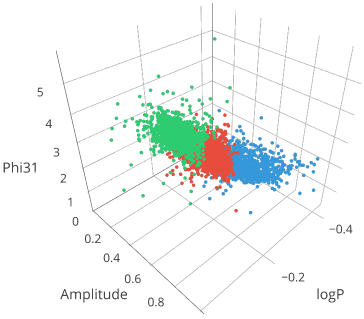
\includegraphics[width=0.5\textwidth]{images/kmeans_01.png}
\end{center}

To create a 3d scatter plot you need to specify the data frame and x,y,z axes. You can also give axes titles as well, in the case that you use shortened versions of the feature names.

\begin{verbatim}
plot_ly(myData, x = ~mag, y = ~amp, z = ~err) %>%
  add_markers() %>%
  layout(scene = list(
    xaxis = list(title = "Magnitude"),
    yaxis = list(title = "Amplitude"),
    zaxis = list(title = "Error")))
\end{verbatim}

If you are trying to plot a lot of data, then you may find the default point sizes to be too large. To decrease the size of the points you can give a \verb|maker| parameter where you specify the size of the points.

\begin{verbatim}
plot_ly(myData, x = ~mag, y = ~amp, z = ~err,
    marker = list(size = 1)) %>%
  add_markers() %>%
  layout(scene = list(
    xaxis = list(title = "Magnitude"),
    yaxis = list(title = "Amplitude"),
    zaxis = list(title = "Error")))
\end{verbatim}

If you want to plot clusters or otherwise color the points based on a feature, you can give a \verb|color| parameter to specify the column to color the points based on. Additionally you can specify the colors to use for the plot by providing a \verb|colors| parameter.

\begin{verbatim}
plot_ly(myData, x = ~mag, y = ~amp, z = ~err, color = ~cluster,
    colors = c("#e74c3c", "#3498db")) %>%
  add_markers() %>%
  layout(scene = list(
    xaxis = list(title = "Magnitude"),
    yaxis = list(title = "Amplitude"),
    zaxis = list(title = "Error")))
\end{verbatim}

\section{Normalizing data}
Before you do any sort of clustering on data, you should first normalize the data. Datasets generally have features that are of different units and ranges of values and this must be taken into account when performing clustering.

To normalize a data frame in R, you can use the \verb|scale| function.

\begin{verbatim}
normalizedData <- scale(myData)
\end{verbatim}

\section{Misc. Functions}

\subsection{Conversion functions}
To convert a numerical factor into the corresponding num representations you can use a combination of the \verb|as.character| and \verb|as.numeric| functions. Any values that are not able to be converted into numeric values will be converted into \verb|NA|s.

\begin{verbatim}
myData$phi31 <- as.numeric(as.character(myData$phi31))
\end{verbatim}

\subsection{Mapping functions}
To map a function over the rows of a data frame and be able to access specific columns you can use the \verb|with| function.

\begin{verbatim}
myData$logMag <- with(myData, log(mag))
\end{verbatim}